\documentclass[11pt,a4paper]{article}
\usepackage[utf8]{inputenc}
\usepackage{amsmath,amssymb,amsfonts}
\usepackage{graphicx}
\usepackage{booktabs}
\usepackage{geometry}
\usepackage{hyperref}
\usepackage{float}
\usepackage{enumitem}
\usepackage{listings}
\usepackage{xcolor}

\geometry{margin=1in}

\lstset{
  basicstyle=\ttfamily\small,
  backgroundcolor=\color{gray!10},
  breaklines=true,
  frame=single,
  language=Python,
}

\title{Introduction to Multimodal Learning\\Problem Set 1 -- Solutions}
\author{}
\date{}

\begin{document}
\maketitle

%=============================================================
\section{Sampling, Aliasing, and DFT}
%=============================================================

\subsection{Nyquist Sampling}

\textbf{1.} The sampling angular frequency must satisfy the \emph{Nyquist condition}:
\[
  \omega_s \geq 2B.
\]
Equivalently, $f_s \geq 2f_{\max}$ where $f_{\max} = B/(2\pi)$.

\textbf{Frequency-domain explanation of aliasing.}
Sampling in the time domain corresponds to periodically replicating the spectrum $X(j\omega)$ with period $\omega_s$.  The sampled spectrum is
\[
  X_s(j\omega) = \frac{1}{T_s}\sum_{k=-\infty}^{\infty} X\bigl(j(\omega - k\omega_s)\bigr).
\]
When $\omega_s < 2B$, adjacent copies of $X(j\omega)$ overlap in frequency.  The overlapping portions add together and cannot be separated, so the original signal cannot be perfectly reconstructed.  This spectral overlap is called \emph{aliasing}.

\medskip
\textbf{2.} An anti-aliasing low-pass filter with cutoff at $\omega_s/2$ is applied \emph{before} sampling.  It removes (or attenuates) all frequency components above $\omega_s/2$, thus ensuring that the signal actually satisfies the Nyquist condition at the chosen sampling rate.  Without this filter, any energy above $\omega_s/2$ would alias into lower frequencies and corrupt the sampled signal.

%--------------------------------------------------
\subsection{A Concrete Aliasing Example}

\textbf{1.} Substituting $t = n/f_s$:
\[
  x[n] = \cos\!\Bigl(\frac{2\pi f_0}{f_s}\,n\Bigr).
\]

\textbf{2.} With $f_0 = 9$ Hz and $f_s = 10$ Hz:
\[
  x[n] = \cos\!\Bigl(\frac{2\pi \cdot 9}{10}\,n\Bigr)
       = \cos\!\Bigl(\frac{9\pi}{5}\,n\Bigr).
\]
Since $\cos\theta = \cos(2\pi - \theta)$, we have
\[
  \cos\!\Bigl(\frac{9\pi}{5}\,n\Bigr)
  = \cos\!\Bigl(2\pi n - \frac{9\pi}{5}\,n\Bigr)
  = \cos\!\Bigl(\frac{\pi}{5}\,n\Bigr)
  = \cos\!\Bigl(\frac{2\pi \cdot 1}{10}\,n\Bigr).
\]
The last expression corresponds to sampling $\cos(2\pi \cdot 1 \cdot t)$ at $f_s = 10$ Hz, i.e.\ a 1\,Hz sinusoid.  Therefore the 9\,Hz and 1\,Hz sinusoids produce \emph{identical} discrete-time samples.

The reason is that $f_0 = 9$ Hz exceeds the Nyquist frequency $f_s/2 = 5$ Hz.  The 9\,Hz component aliases to $f_s - f_0 = 10 - 9 = 1$ Hz, making the two signals indistinguishable after sampling.

%--------------------------------------------------
\subsection{DFT, Windowing, and FFT}

\textbf{1.} The DTFT produces a \emph{continuous} function of frequency $\omega$, which requires infinitely many values to represent.  A computer can only store and compute finitely many numbers.  The DFT evaluates the spectrum at $N$ discrete, equally-spaced frequency bins, yielding a finite-length vector that can be stored, manipulated, and inverted exactly on a computer.

\medskip
\textbf{2.} Truncating a signal to $N$ samples is equivalent to multiplying by a rectangular window $w[n]$.  In the frequency domain this corresponds to \emph{convolving} the true spectrum with the DFT of the rectangular window (a Dirichlet kernel / sinc-like function).  The Dirichlet kernel has a narrow main lobe but significant side lobes.  This convolution causes \emph{spectral leakage}: energy from each true frequency component spreads into neighboring bins, distorting the frequency-domain result and making it harder to resolve closely spaced spectral peaks.

\medskip
\textbf{3.} The Hann window tapers smoothly to zero at both ends.  Its frequency-domain counterpart has much lower side lobes compared to the rectangular window (at the cost of a slightly wider main lobe).  The reduced side lobes greatly suppress spectral leakage, giving a cleaner spectrum that better reveals the true frequency content in many practical scenarios.

\medskip
\textbf{4.} \begin{itemize}[nosep]
  \item \textbf{Direct DFT:} Computing $N$ frequency bins, each a sum of $N$ terms, requires $O(N^2)$ complex multiplications and additions.
  \item \textbf{FFT (Cooley--Tukey):} Exploits the symmetry and periodicity of the twiddle factors to decompose the $N$-point DFT into smaller DFTs recursively, reducing the complexity to $O(N \log N)$.
\end{itemize}
For large $N$ the FFT is dramatically faster; for example, at $N=1024$ the speedup is roughly $1024/10 \approx 100\times$.

%=============================================================
\section{Image Compression Fundamentals}
%=============================================================

\subsection{DCT vs.\ DFT}

The DCT is preferred over the DFT for image compression for at least two reasons:

\begin{enumerate}[nosep]
  \item \textbf{Real-valued coefficients.}  The DCT of a real signal is purely real, whereas the DFT produces complex coefficients.  Working with real numbers halves the storage and avoids the need to store phase information.
  \item \textbf{Better energy compaction.}  For typical natural image blocks, the DCT concentrates more energy into fewer low-frequency coefficients than the DFT.  This is because the DCT implicitly assumes an even (symmetric) extension of the block at its boundaries, avoiding the sharp discontinuity that a periodic extension (as assumed by the DFT) would create at the block edges.  Fewer significant coefficients mean higher compression efficiency after quantization.
\end{enumerate}

%--------------------------------------------------
\subsection{Quantization}

\textbf{1.} Quantization is the \emph{lossy} step in the compression pipeline.  It maps the continuous-valued (or finely-valued) DCT coefficients to a smaller set of discrete levels by dividing each coefficient by the corresponding entry of a quantization matrix and rounding to the nearest integer.  This drastically reduces the number of distinct values (producing many zeros, especially in high-frequency positions), which enables efficient entropy coding downstream.

\medskip
\textbf{2.} The human visual system (HVS) is much less sensitive to high-frequency detail (fine textures, sharp edges) than to low-frequency content (smooth gradients, overall brightness).  By quantizing high-frequency coefficients more coarsely (using larger quantization step sizes), we lose information that is perceptually less important, achieving higher compression with minimal visible quality loss.

%--------------------------------------------------
\subsection{Codeword Assignment}

\textbf{1.} Variable-length coding assigns shorter binary codewords to more frequently occurring symbols and longer codewords to rarer symbols.  This minimizes the expected (average) code length, bringing it close to the entropy of the source.

\medskip
\textbf{2.} The code must satisfy the \emph{prefix-free} (or ``prefix'') property: no codeword is a prefix of any other codeword.  This ensures that the decoder can parse the bitstream unambiguously from left to right without needing delimiters or look-ahead.

\medskip
\textbf{3.} Huffman coding is an optimal prefix-free code.  By construction (greedily merging the two least probable symbols at each step), it assigns shorter codewords to higher-probability symbols.  This minimizes the weighted average code length $\bar{L} = \sum_i p_i \, l_i$, achieving compression close to the source entropy $H$.

%--------------------------------------------------
\subsection{JPEG Color Space}

\textbf{1.} Converting from RGB to YCbCr separates \emph{luminance} (Y, perceived brightness) from \emph{chrominance} (Cb, Cr, color difference signals).  This is useful because:
\begin{itemize}[nosep]
  \item The three RGB channels are highly correlated; YCbCr decorrelates them, making independent compression of each channel more efficient.
  \item It aligns the representation with the properties of human vision, facilitating perceptually optimized compression.
\end{itemize}

\medskip
\textbf{2.} The chrominance channels (Cb and Cr) can be compressed more aggressively.  The HVS has much higher spatial resolution for luminance than for color.  Therefore, the Cb and Cr channels are typically subsampled (e.g., 4:2:0) and quantized more coarsely with little perceptible quality loss, while the luminance channel Y is preserved at higher fidelity.

%=============================================================
\section{Programming: Mini JPEG-Style Compressor}
%=============================================================

The complete implementation is in \texttt{mini\_jpeg.py}.  Below we present the results.

\subsection{Patch-wise DCT (3.1)}

We select four representative $8\times 8$ patches from each image at different variance levels (high-variance = textured, low-variance = smooth).  Figures~\ref{fig:loc1}--\ref{fig:loc2} show where the patches are located on the original image.  Figures~\ref{fig:dct1}--\ref{fig:dct2} show each patch zoomed in (top row) alongside its DCT log-magnitude (bottom row).

\begin{figure}[H]
  \centering
  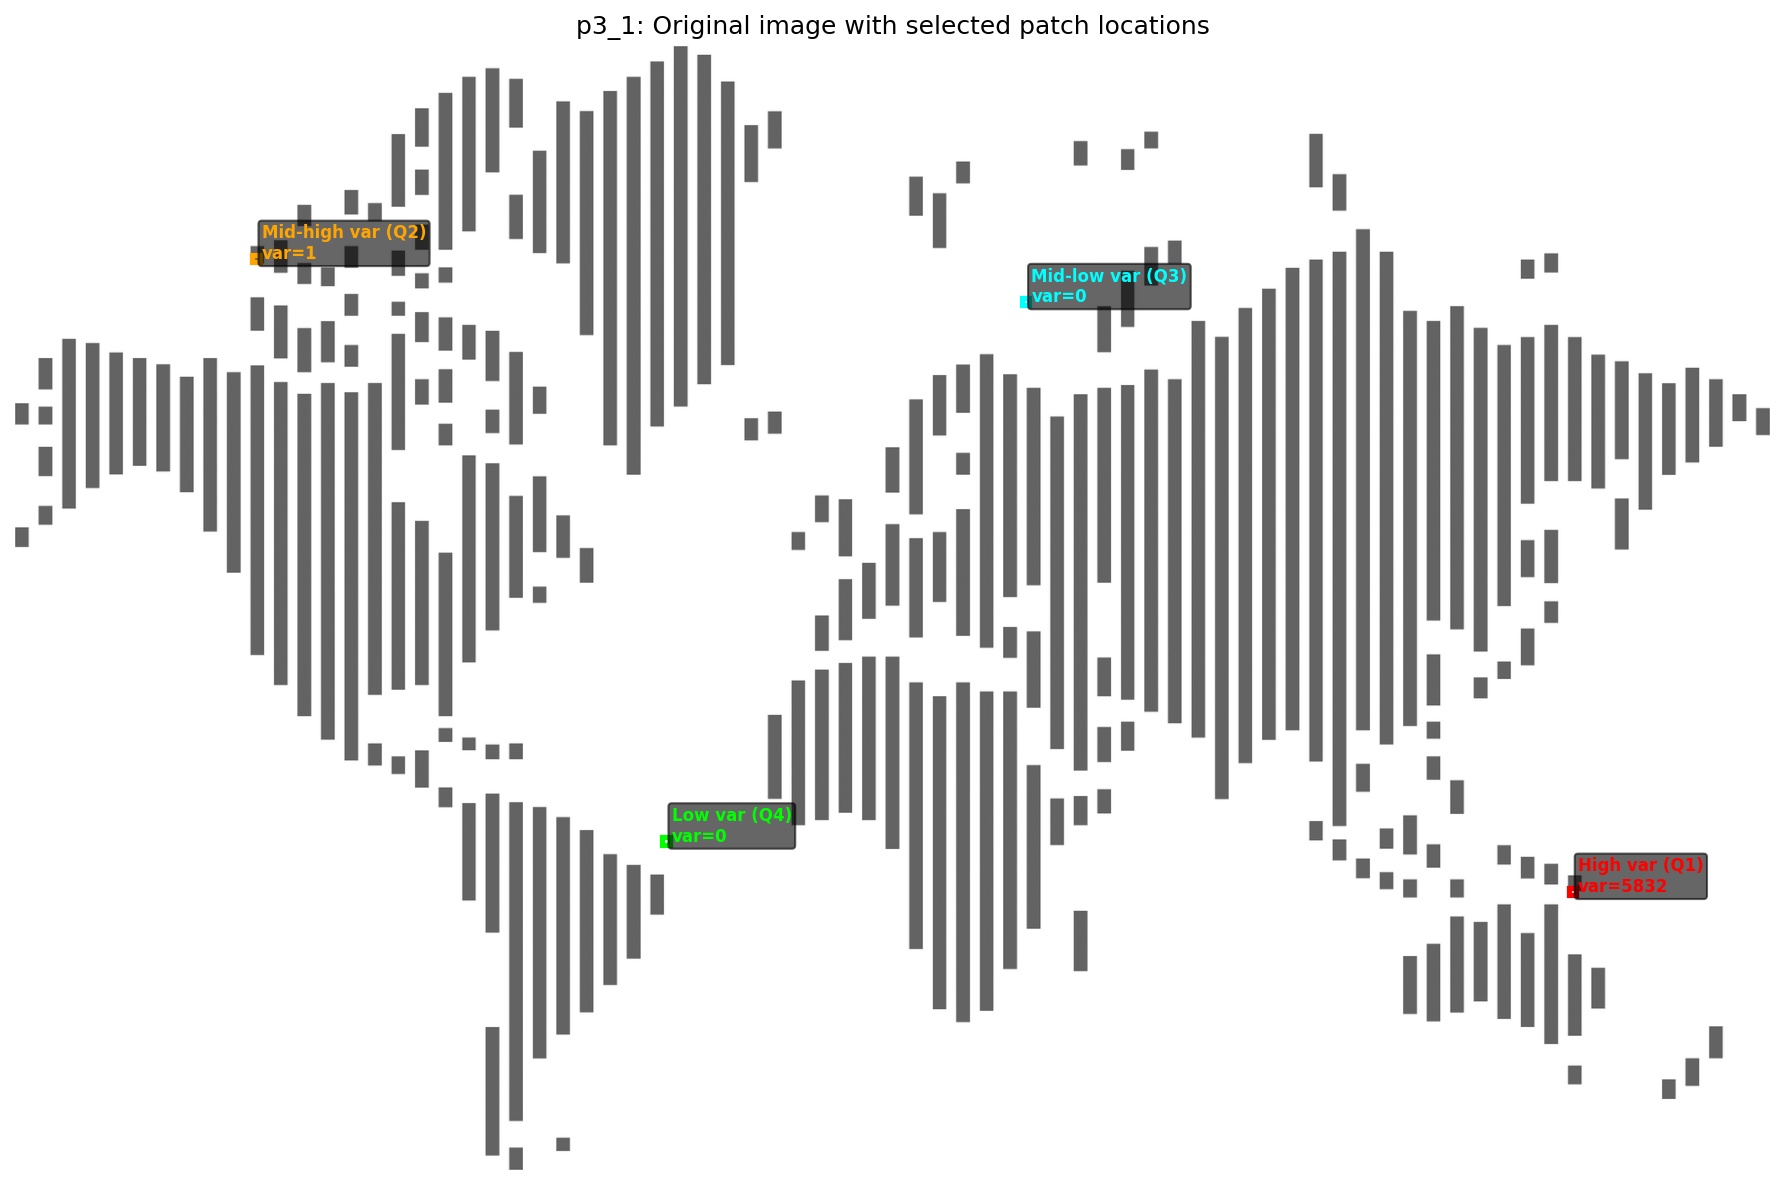
\includegraphics[width=0.85\textwidth]{figures/p3_1_patch_locations.png}
  \caption{\texttt{p3\_1.png}: Original image with selected patch locations highlighted by colored boxes.}
  \label{fig:loc1}
\end{figure}

\begin{figure}[H]
  \centering
  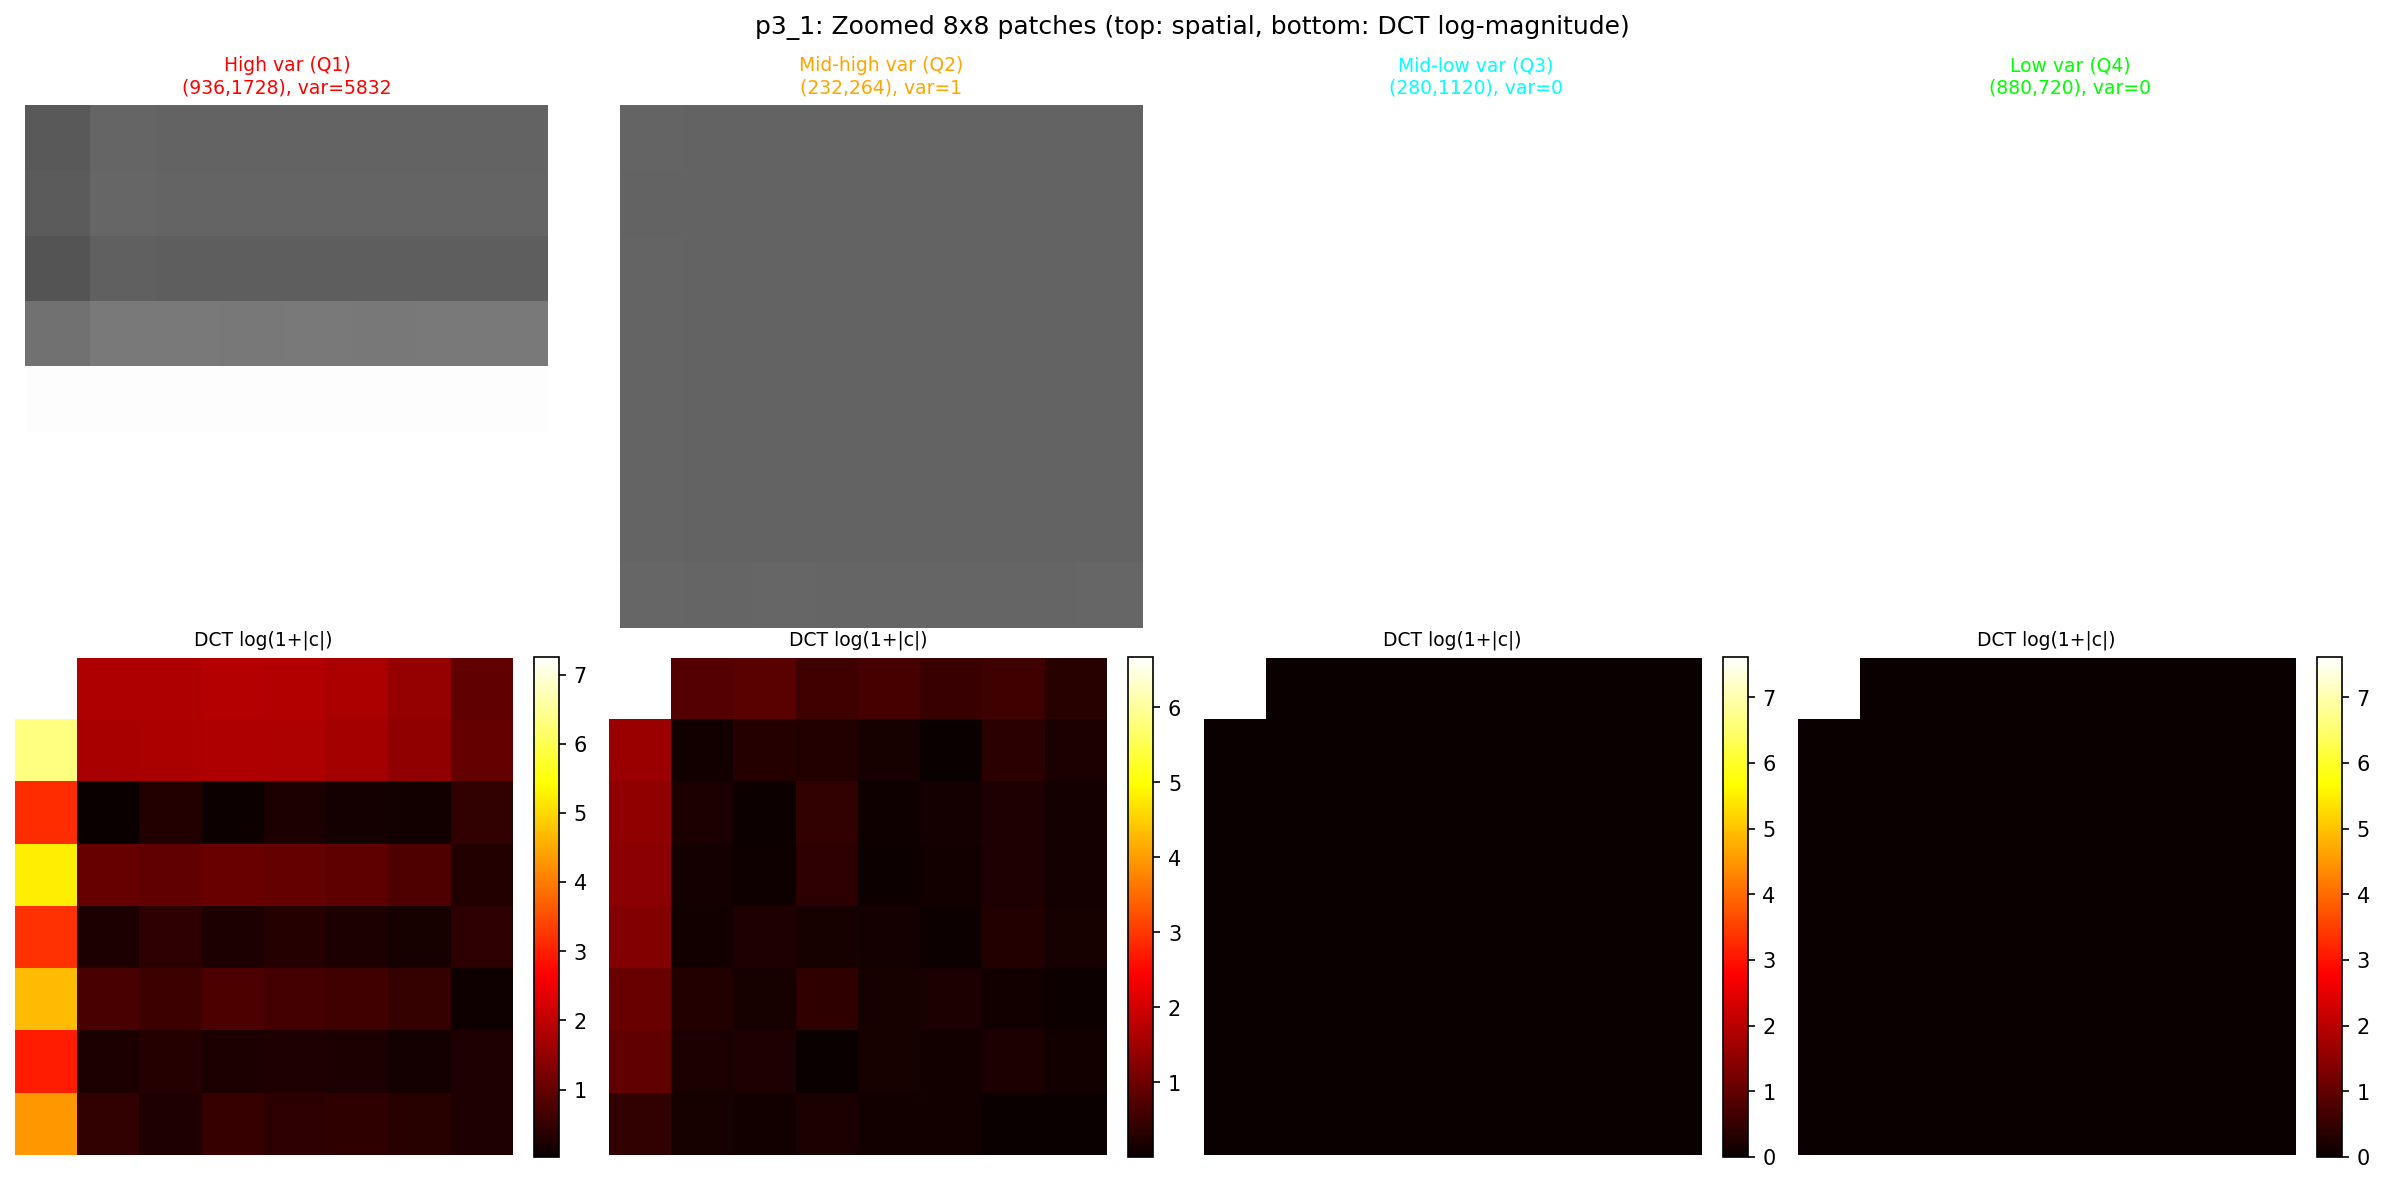
\includegraphics[width=0.85\textwidth]{figures/p3_1_dct_patches.png}
  \caption{\texttt{p3\_1.png}: Zoomed $8\times 8$ patches (top: spatial domain, bottom: DCT $\log(1+|c|)$). Colors match Figure~\ref{fig:loc1}.}
  \label{fig:dct1}
\end{figure}

\begin{figure}[H]
  \centering
  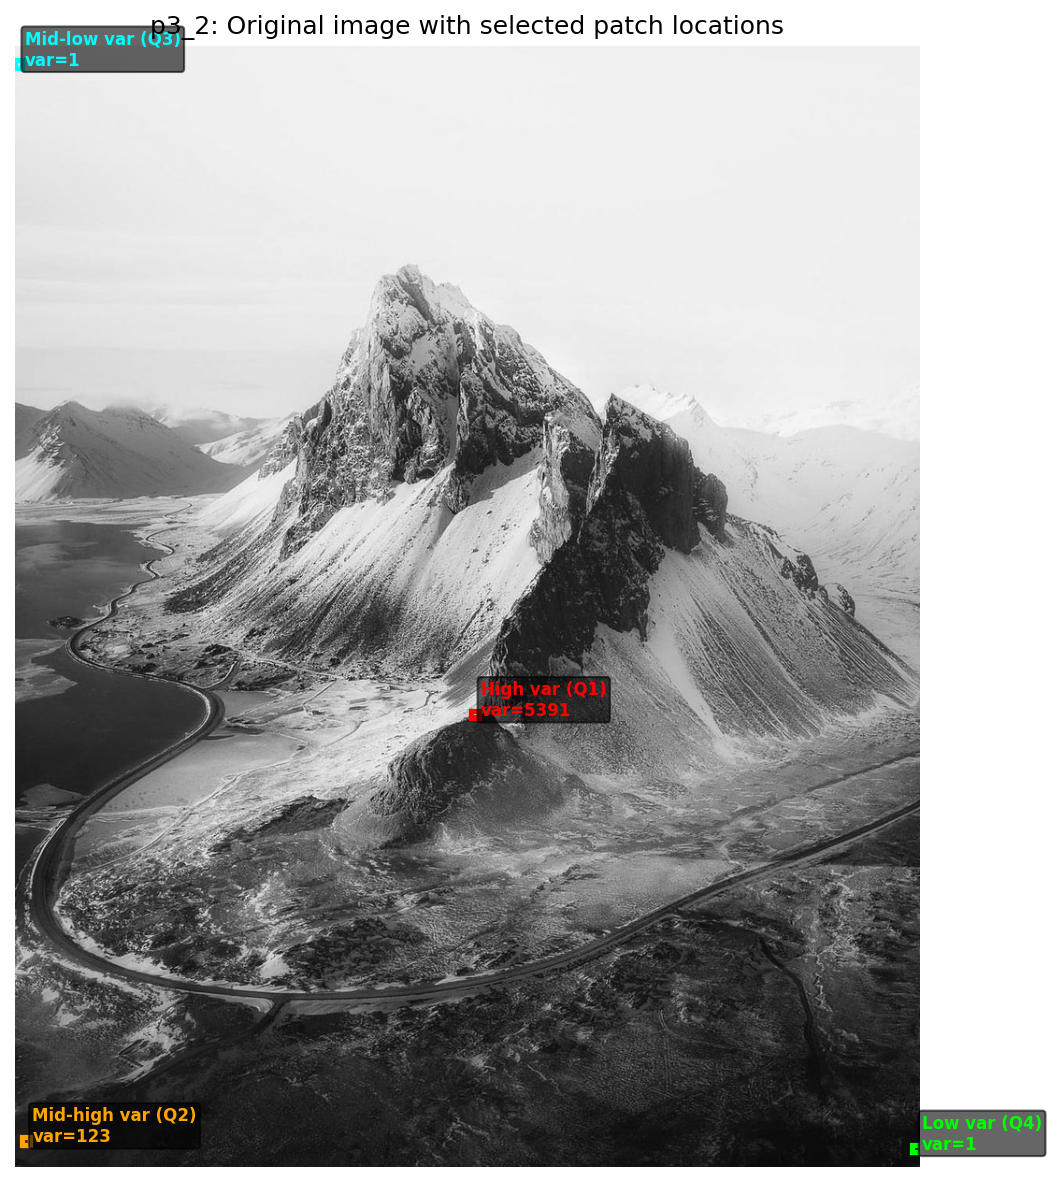
\includegraphics[width=0.85\textwidth]{figures/p3_2_patch_locations.png}
  \caption{\texttt{p3\_2.png}: Original image with selected patch locations highlighted by colored boxes.}
  \label{fig:loc2}
\end{figure}

\begin{figure}[H]
  \centering
  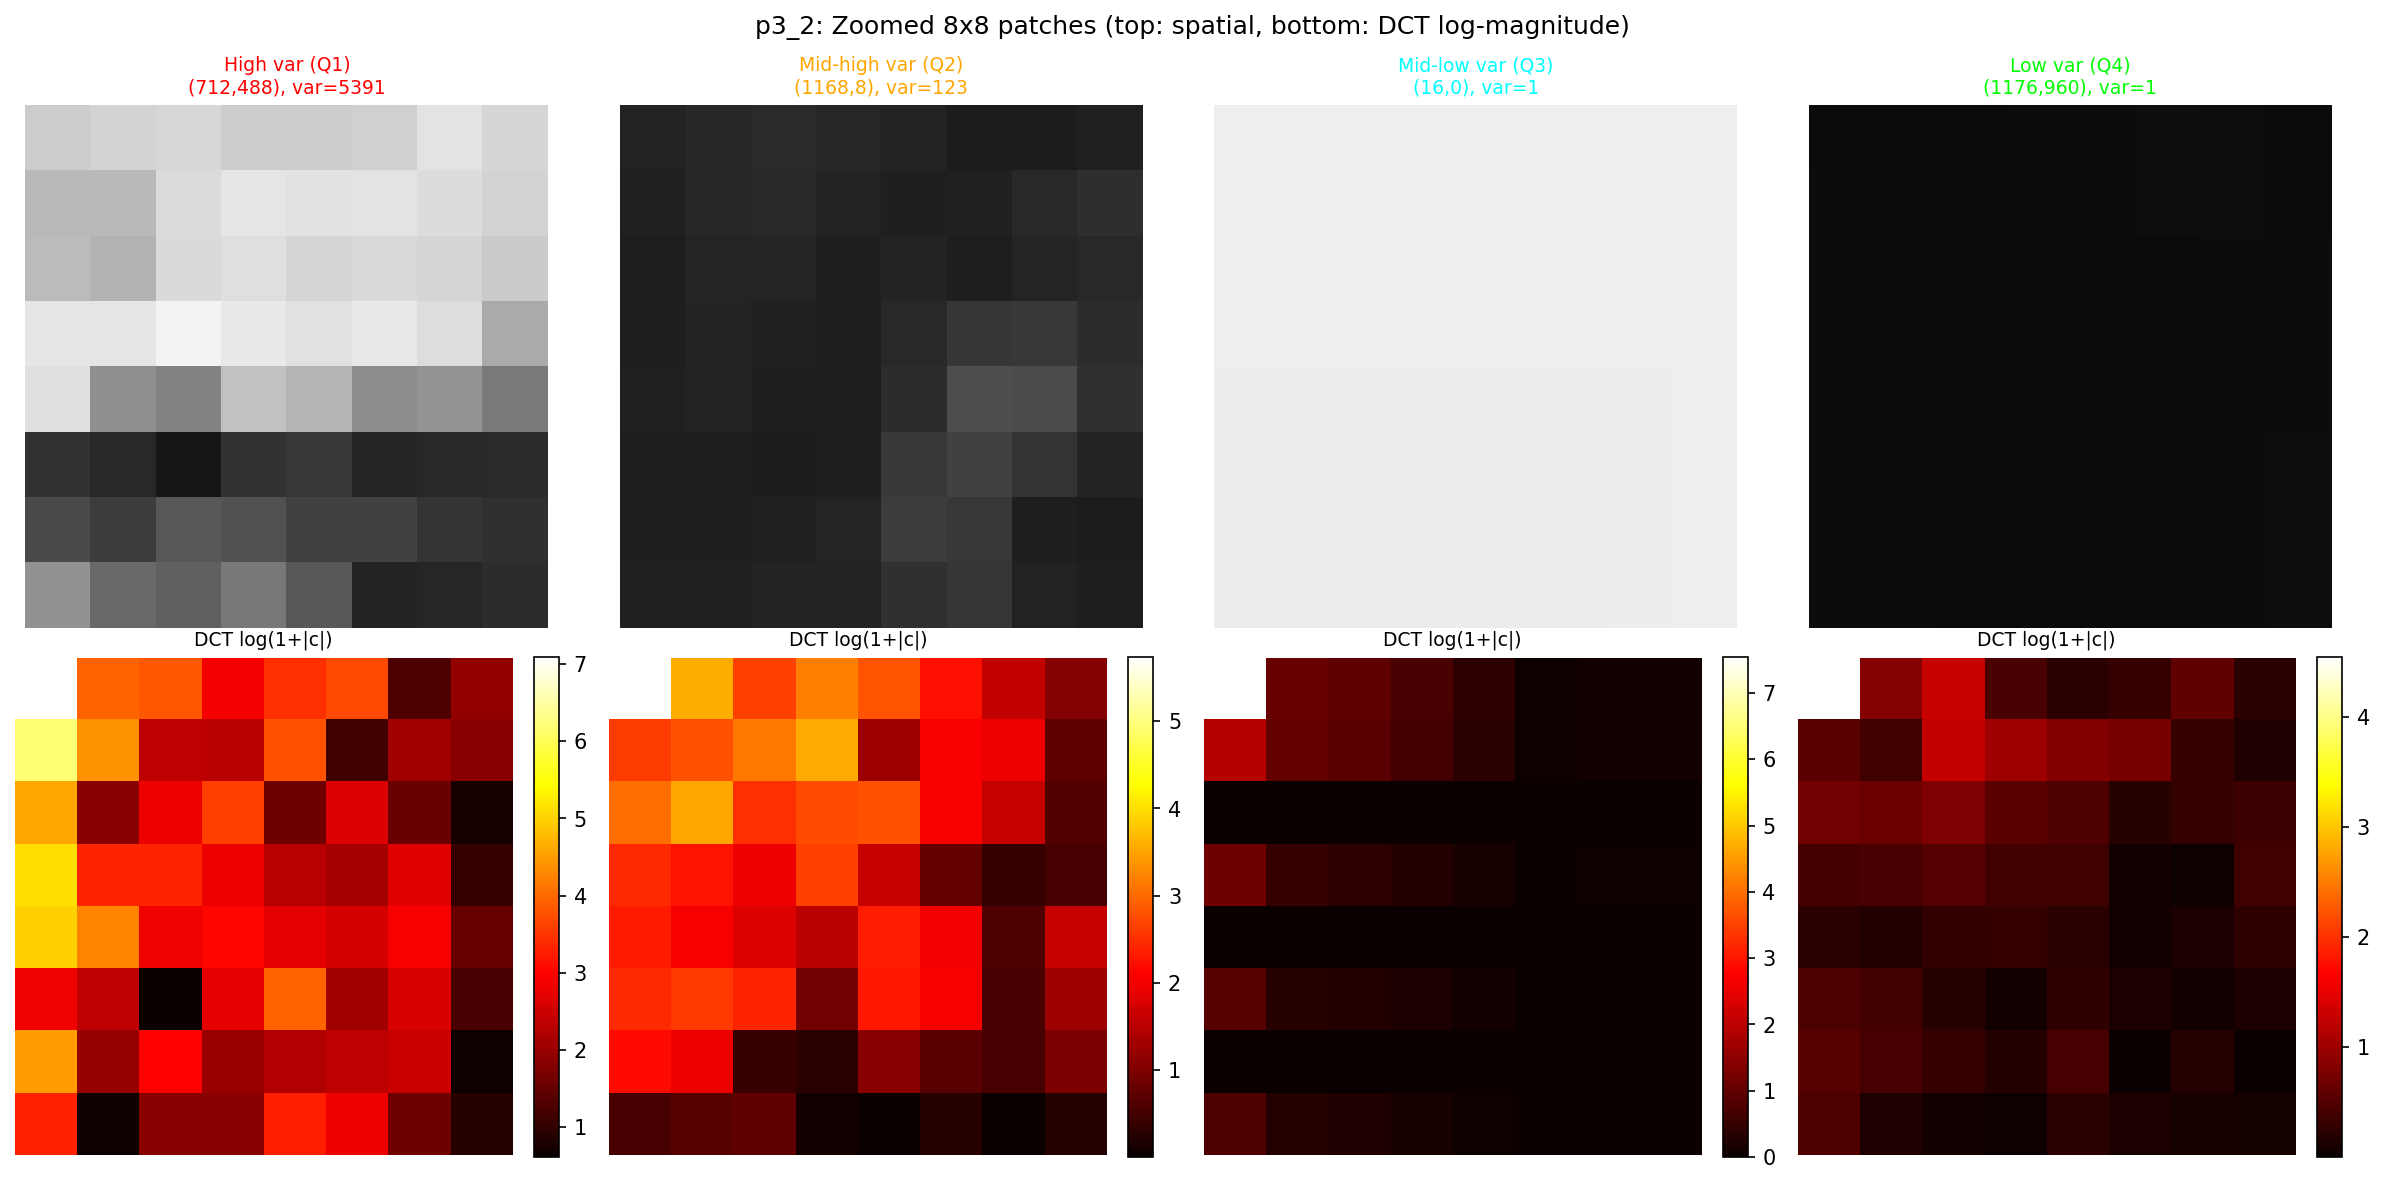
\includegraphics[width=0.85\textwidth]{figures/p3_2_dct_patches.png}
  \caption{\texttt{p3\_2.png}: Zoomed $8\times 8$ patches (top: spatial domain, bottom: DCT $\log(1+|c|)$). Colors match Figure~\ref{fig:loc2}.}
  \label{fig:dct2}
\end{figure}

\textbf{Observation:}
\begin{itemize}[nosep]
  \item \textbf{High-variance patches} (textured regions with edges/gradients) have DCT energy spread across many frequencies --- the heat map is broadly lit.
  \item \textbf{Low-variance patches} (smooth/uniform regions) have nearly all energy concentrated in the DC component (top-left corner) --- the rest of the heat map is dark.
  \item For \texttt{p3\_1.png} (a stylized map graphic), the majority of patches are uniform, so energy compaction is extreme.  For \texttt{p3\_2.png} (a natural photograph with rich texture), more patches retain mid/high-frequency energy.
\end{itemize}
This demonstrates why DCT-based compression works: smooth regions (common in most images) produce sparse coefficient blocks that are highly compressible after quantization.

%--------------------------------------------------
\subsection{Quantization Design (3.2)}

\subsubsection*{Strategy A: Simple Frequency-Dependent Quantization}

Figures~\ref{fig:a4}--\ref{fig:a16} show the original and reconstructed images under the simple quantization matrix $Q(i,j) = p(i+j+1)$ for $p\in\{4,8,16\}$.

\begin{figure}[H]
  \centering
  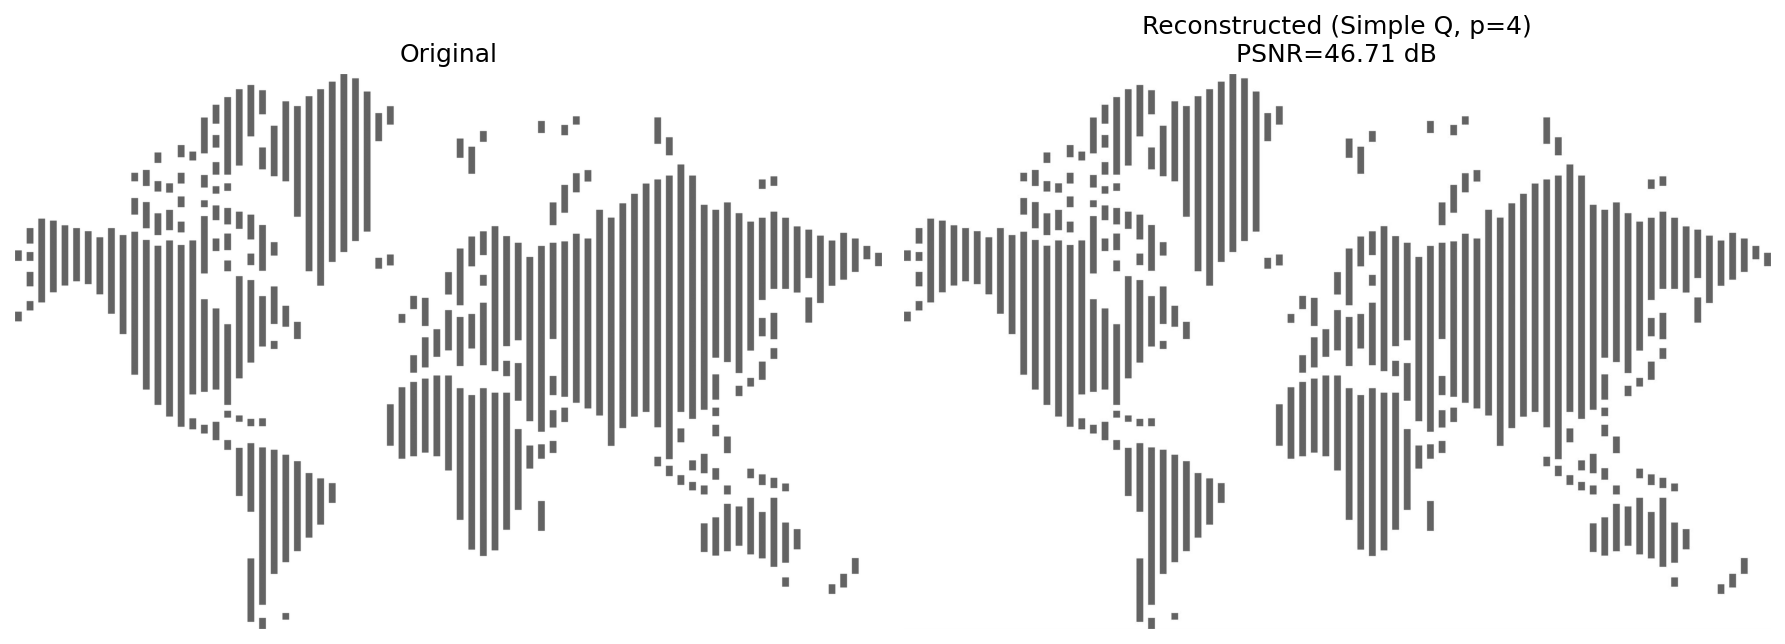
\includegraphics[width=0.48\textwidth]{figures/p3_1_A_p4.png}
  \hfill
  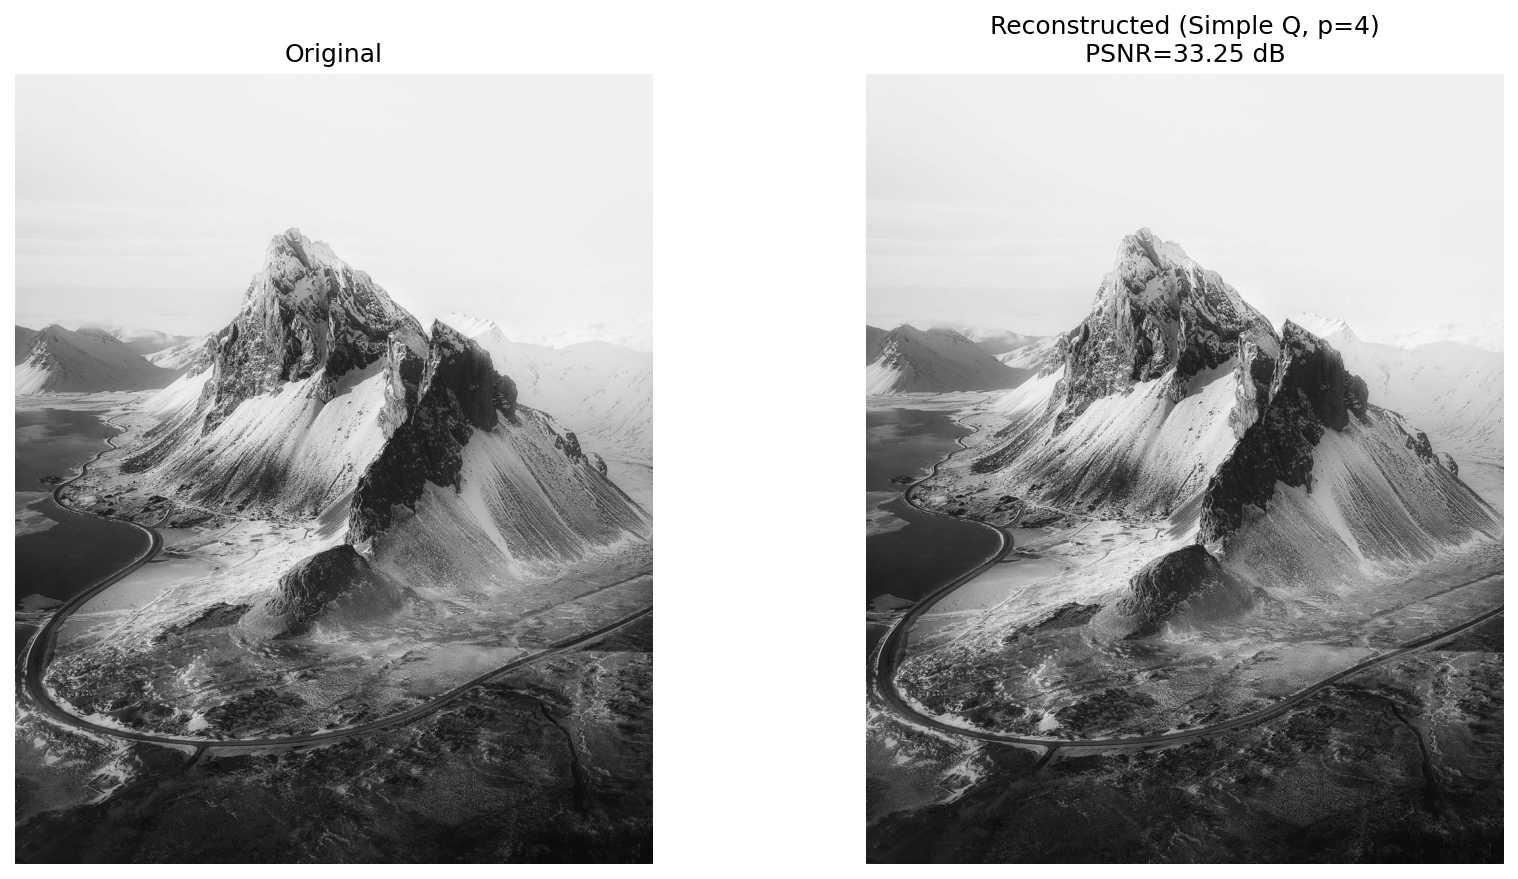
\includegraphics[width=0.48\textwidth]{figures/p3_2_A_p4.png}
  \caption{Reconstruction with Simple Q, $p=4$.}
  \label{fig:a4}
\end{figure}

\begin{figure}[H]
  \centering
  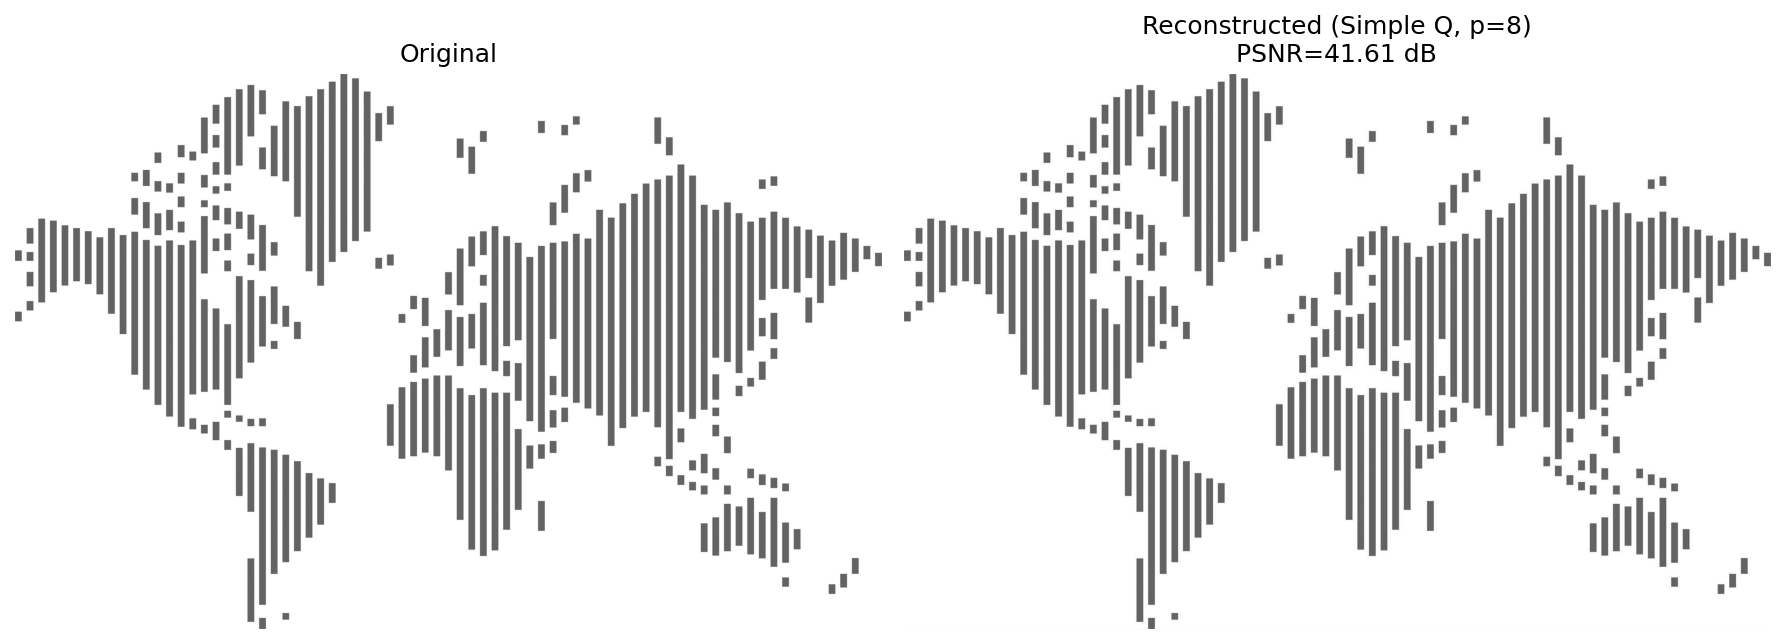
\includegraphics[width=0.48\textwidth]{figures/p3_1_A_p8.png}
  \hfill
  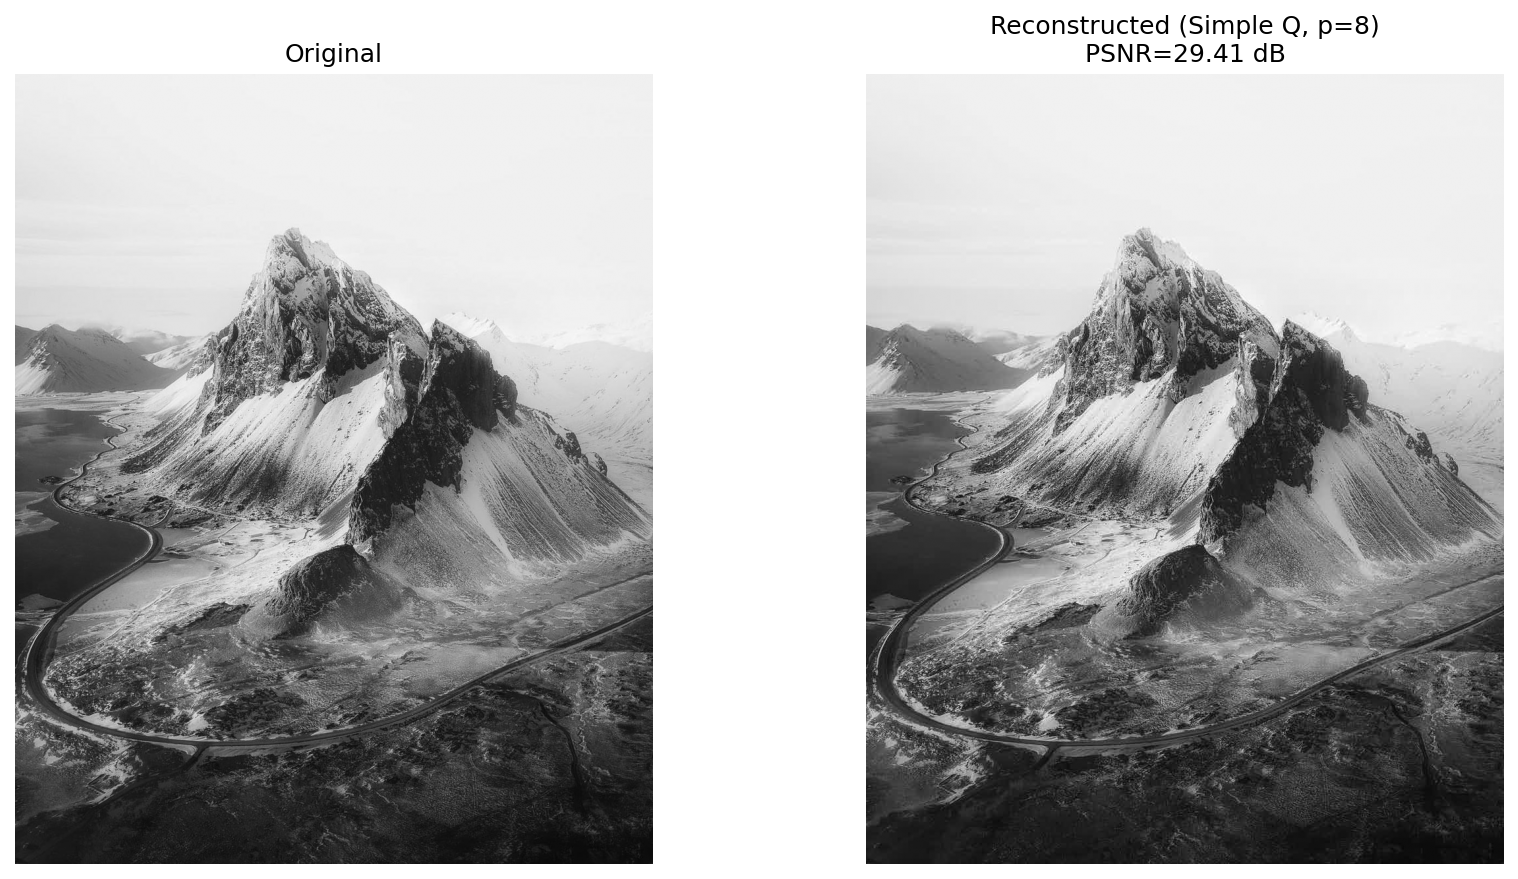
\includegraphics[width=0.48\textwidth]{figures/p3_2_A_p8.png}
  \caption{Reconstruction with Simple Q, $p=8$.}
  \label{fig:a8}
\end{figure}

\begin{figure}[H]
  \centering
  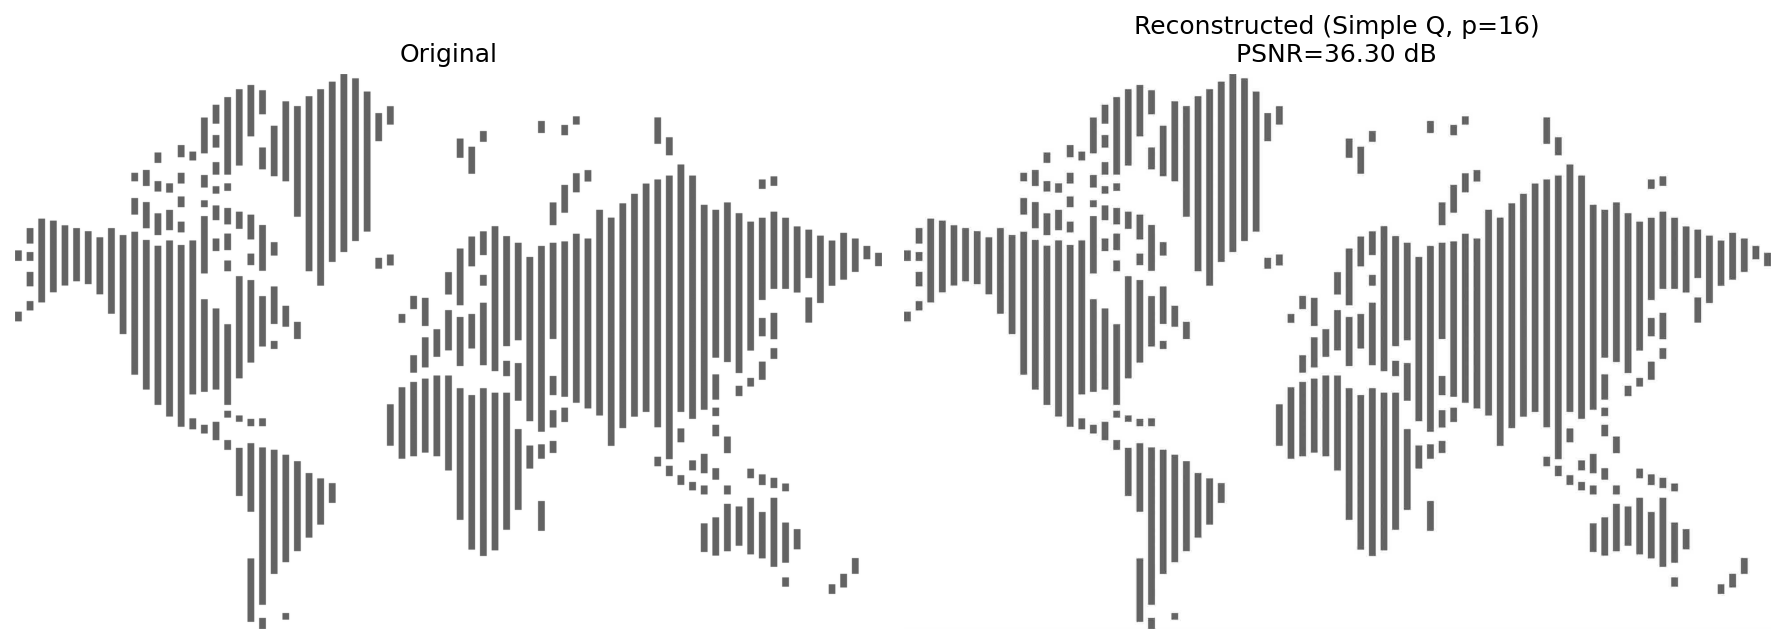
\includegraphics[width=0.48\textwidth]{figures/p3_1_A_p16.png}
  \hfill
  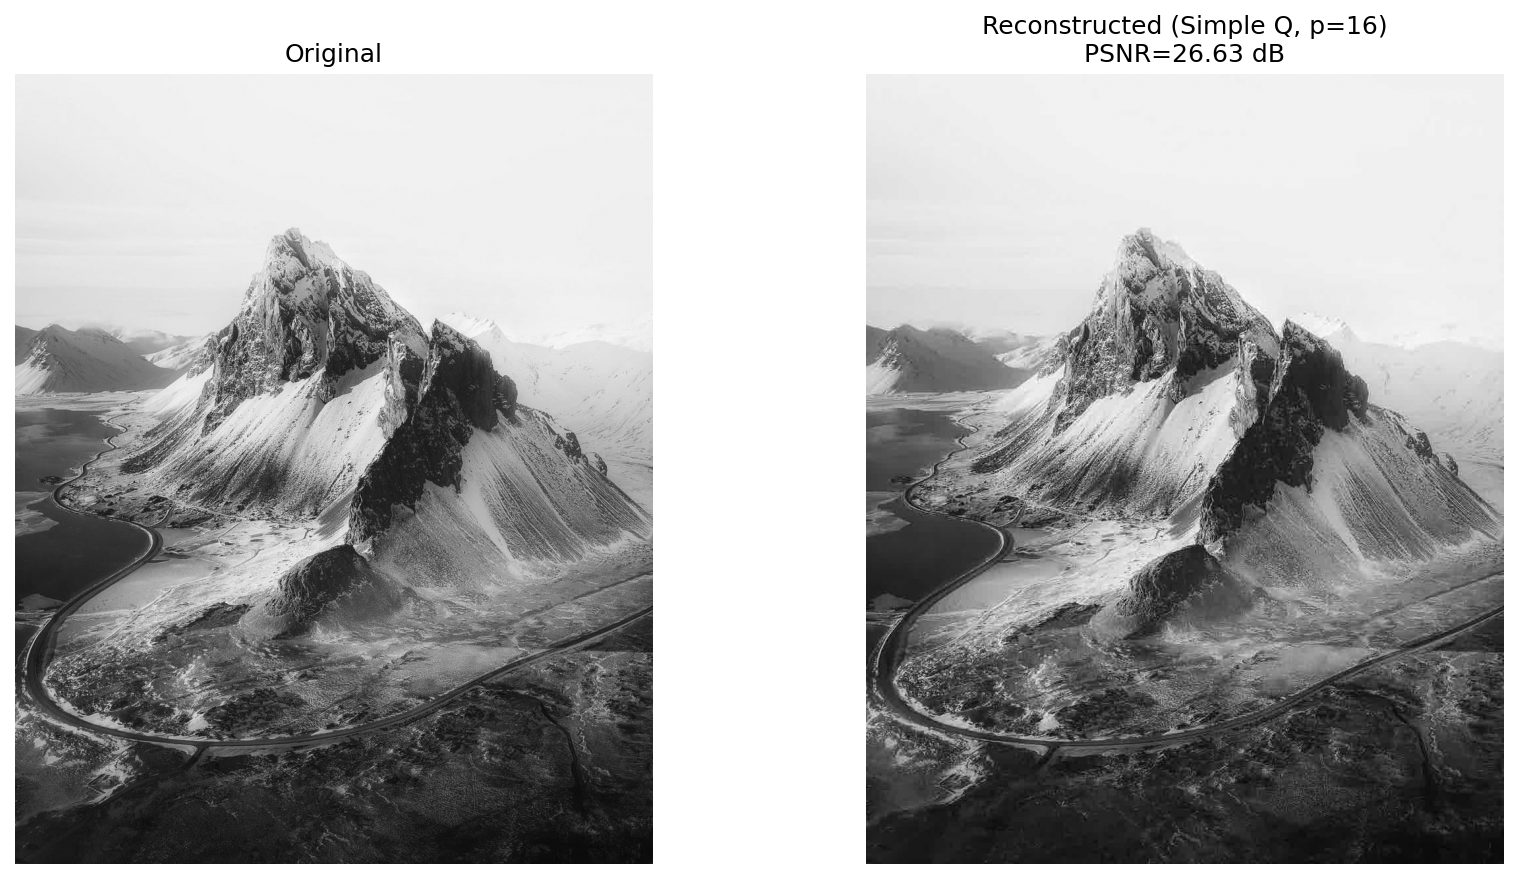
\includegraphics[width=0.48\textwidth]{figures/p3_2_A_p16.png}
  \caption{Reconstruction with Simple Q, $p=16$.}
  \label{fig:a16}
\end{figure}

\subsubsection*{Strategy B: JPEG Luminance Quantization Matrix}

Figures~\ref{fig:b05}--\ref{fig:b2} show results using $pQ_Y$ for $p\in\{0.5, 1, 2\}$.

\begin{figure}[H]
  \centering
  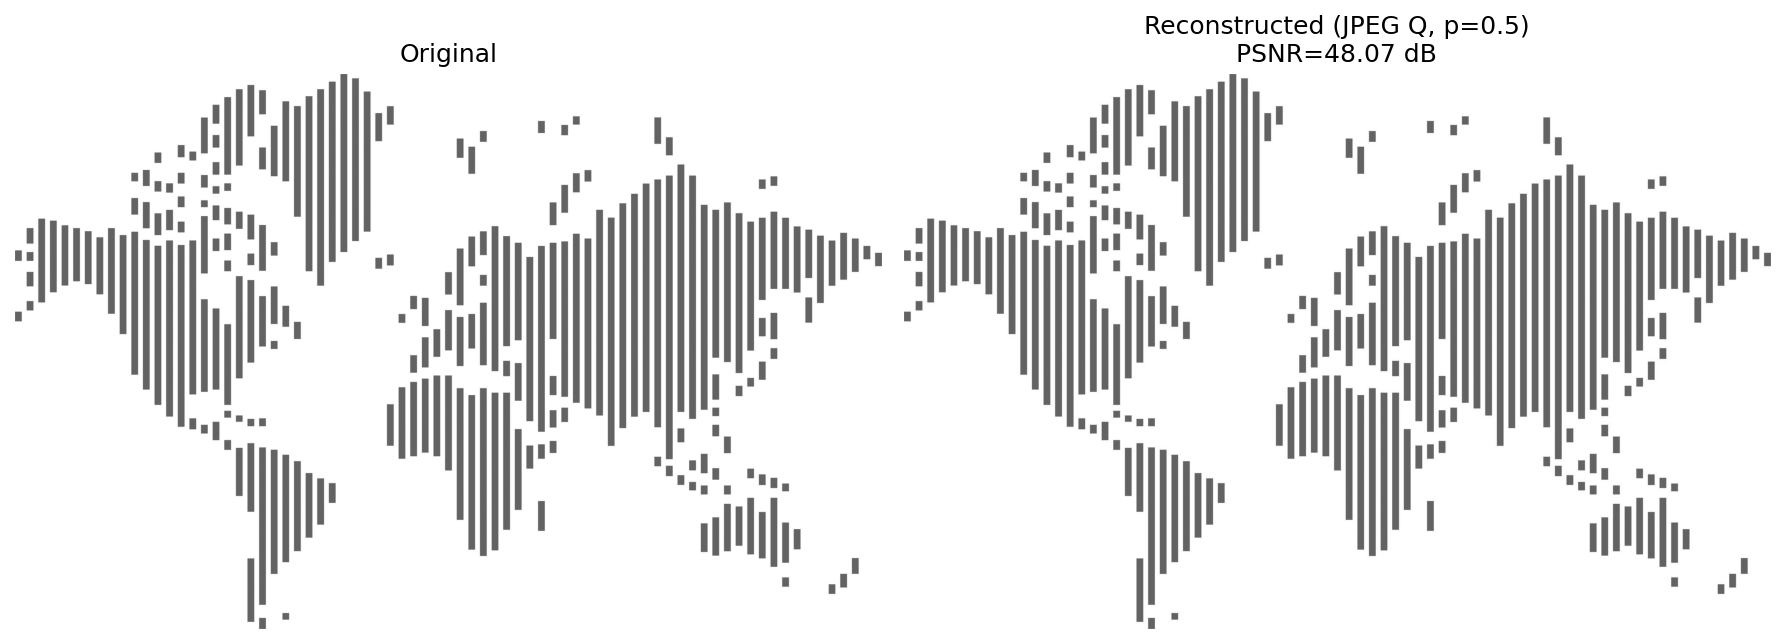
\includegraphics[width=0.48\textwidth]{figures/p3_1_B_p0_5.png}
  \hfill
  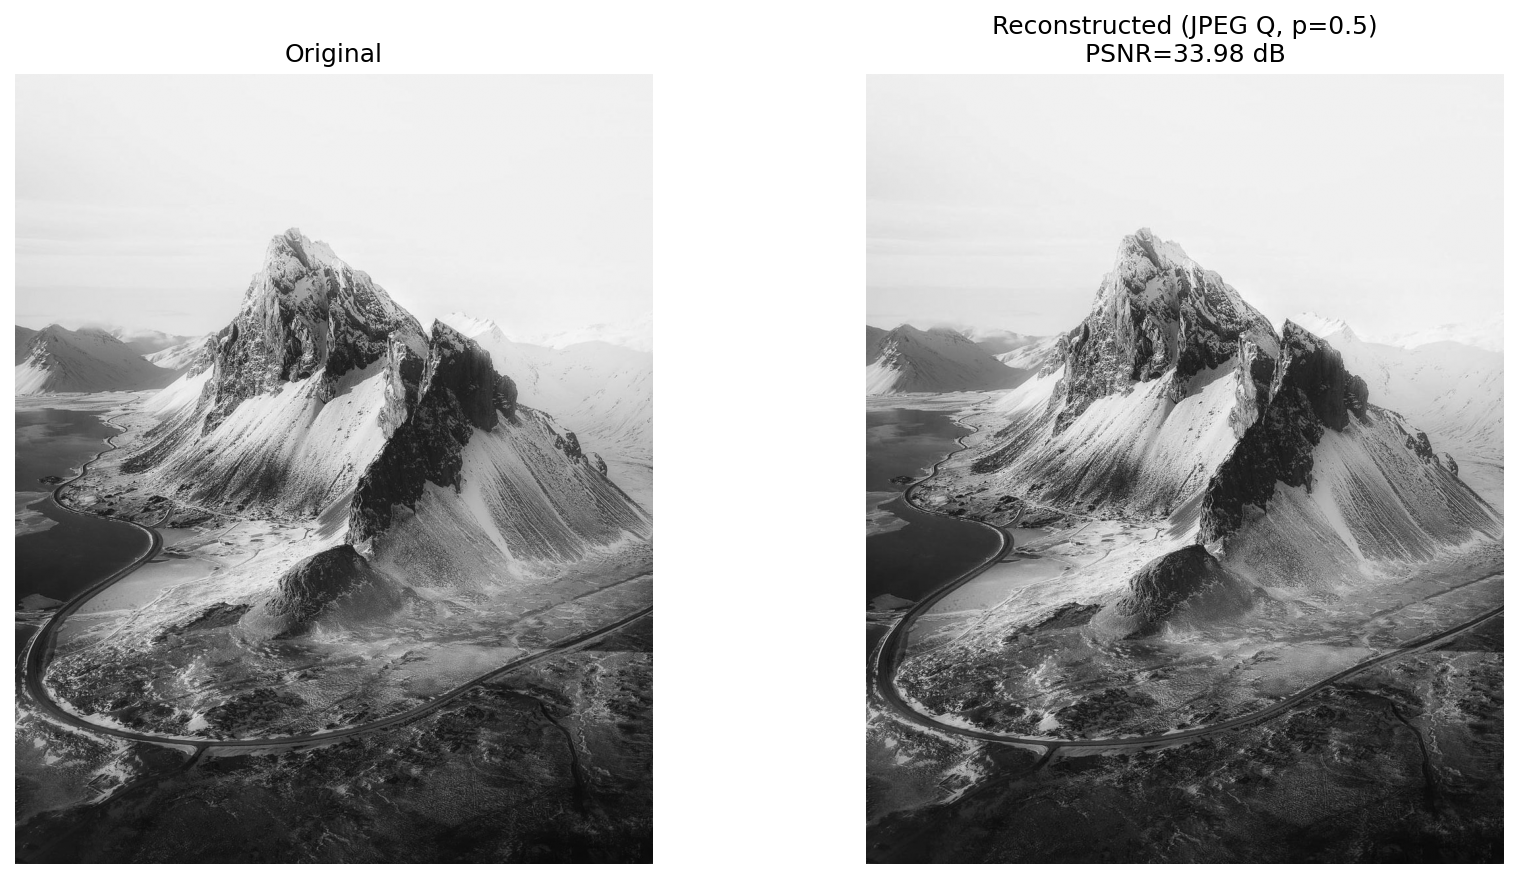
\includegraphics[width=0.48\textwidth]{figures/p3_2_B_p0_5.png}
  \caption{Reconstruction with JPEG $Q_Y$, $p=0.5$.}
  \label{fig:b05}
\end{figure}

\begin{figure}[H]
  \centering
  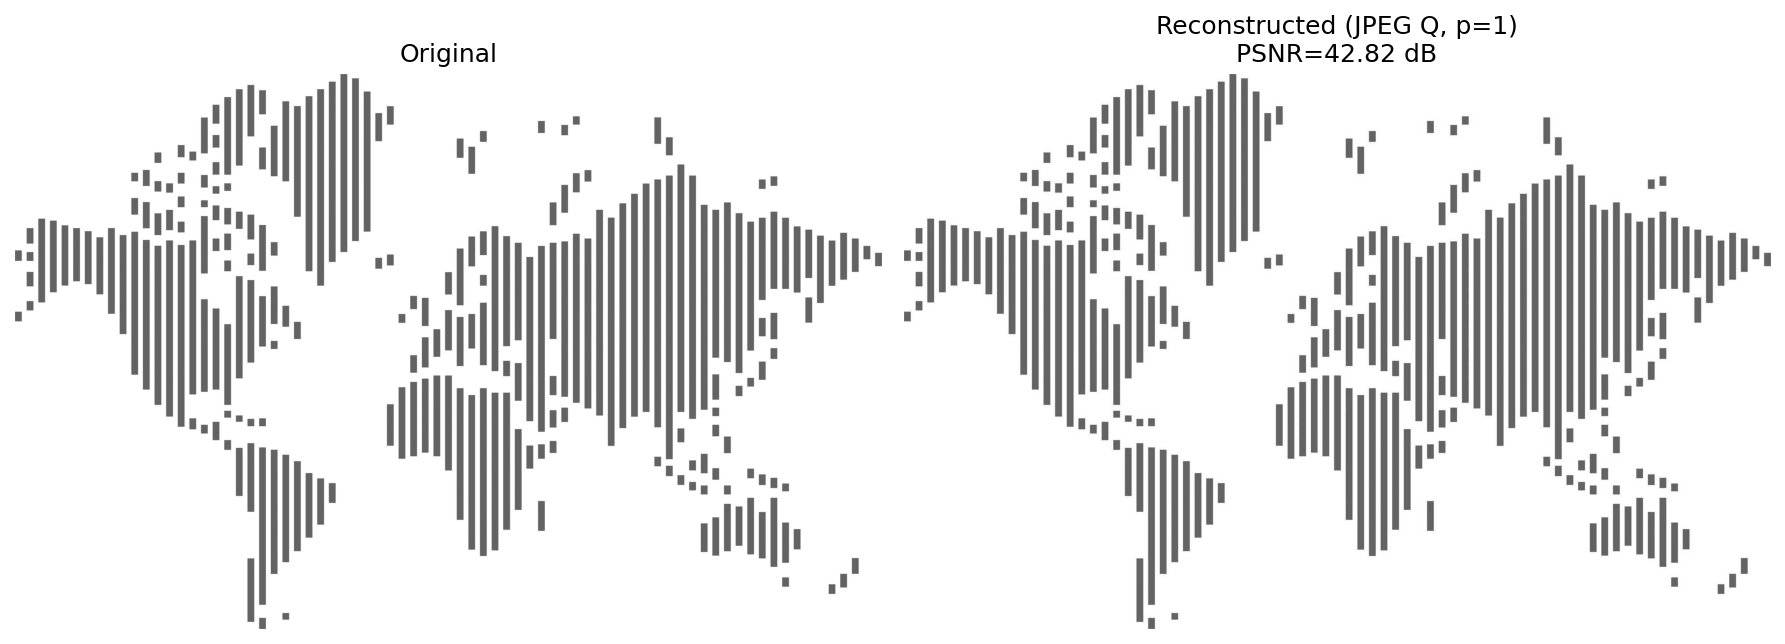
\includegraphics[width=0.48\textwidth]{figures/p3_1_B_p1.png}
  \hfill
  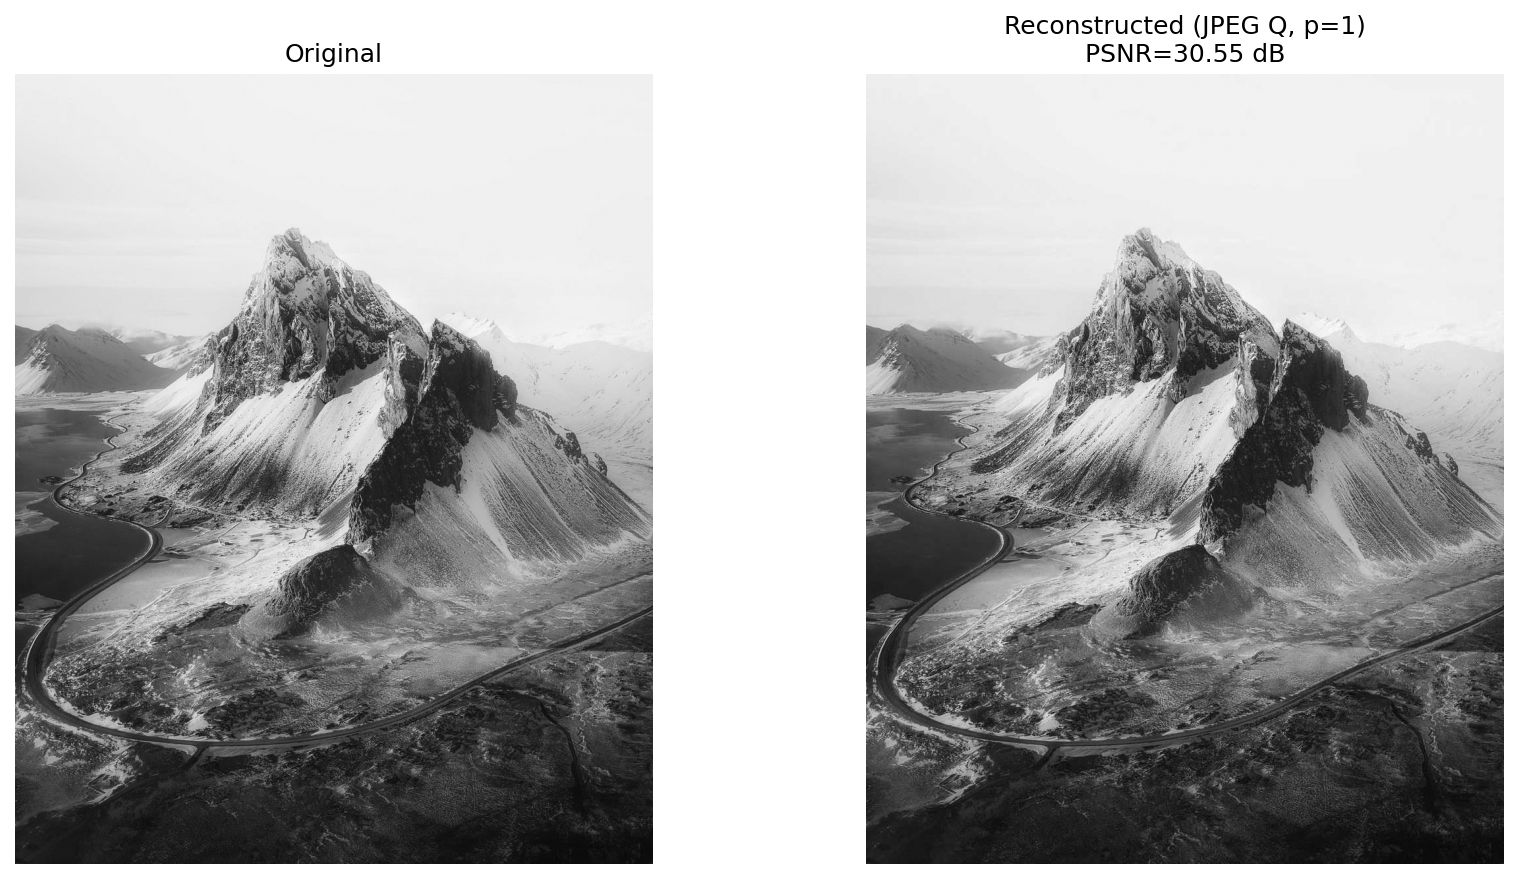
\includegraphics[width=0.48\textwidth]{figures/p3_2_B_p1.png}
  \caption{Reconstruction with JPEG $Q_Y$, $p=1$.}
  \label{fig:b2a}
\end{figure}

\begin{figure}[H]
  \centering
  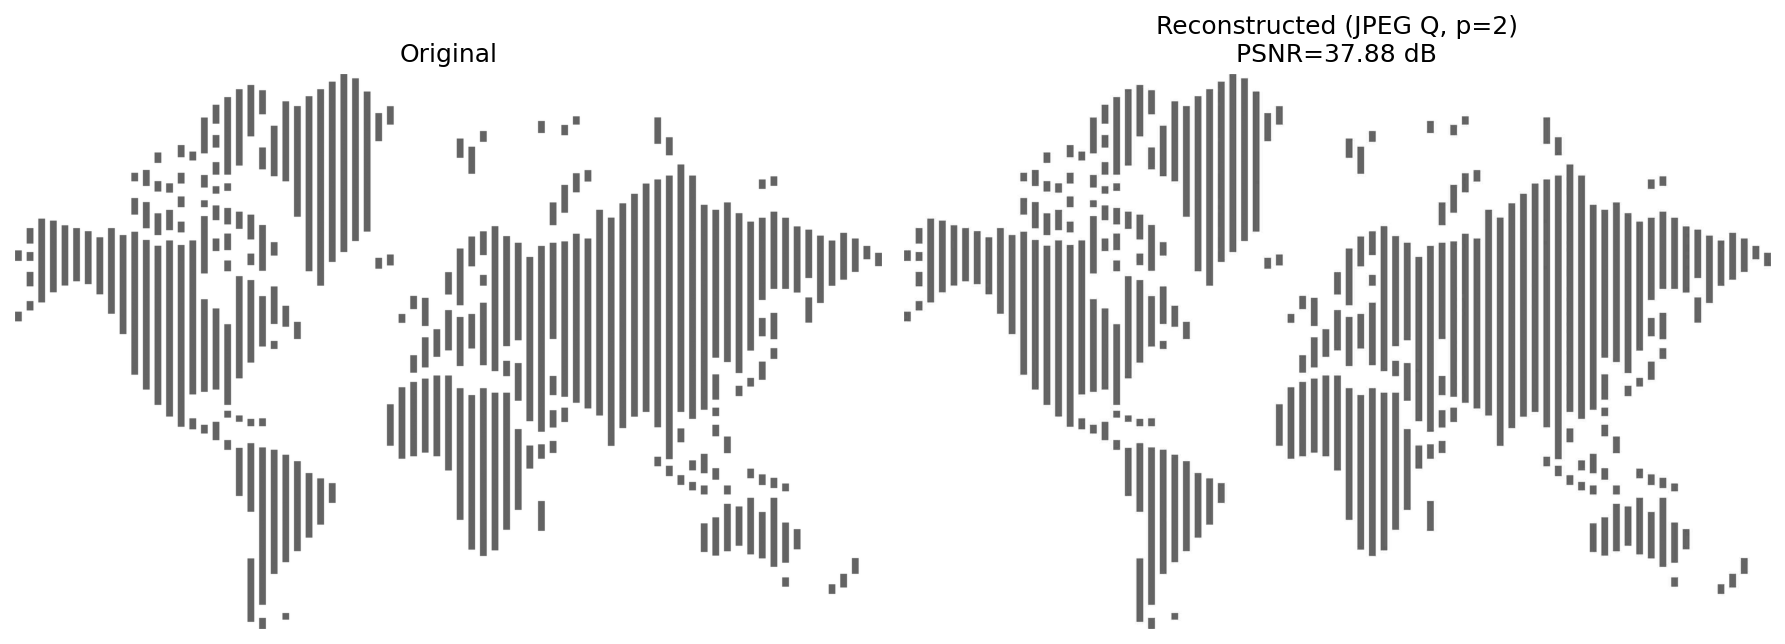
\includegraphics[width=0.48\textwidth]{figures/p3_1_B_p2.png}
  \hfill
  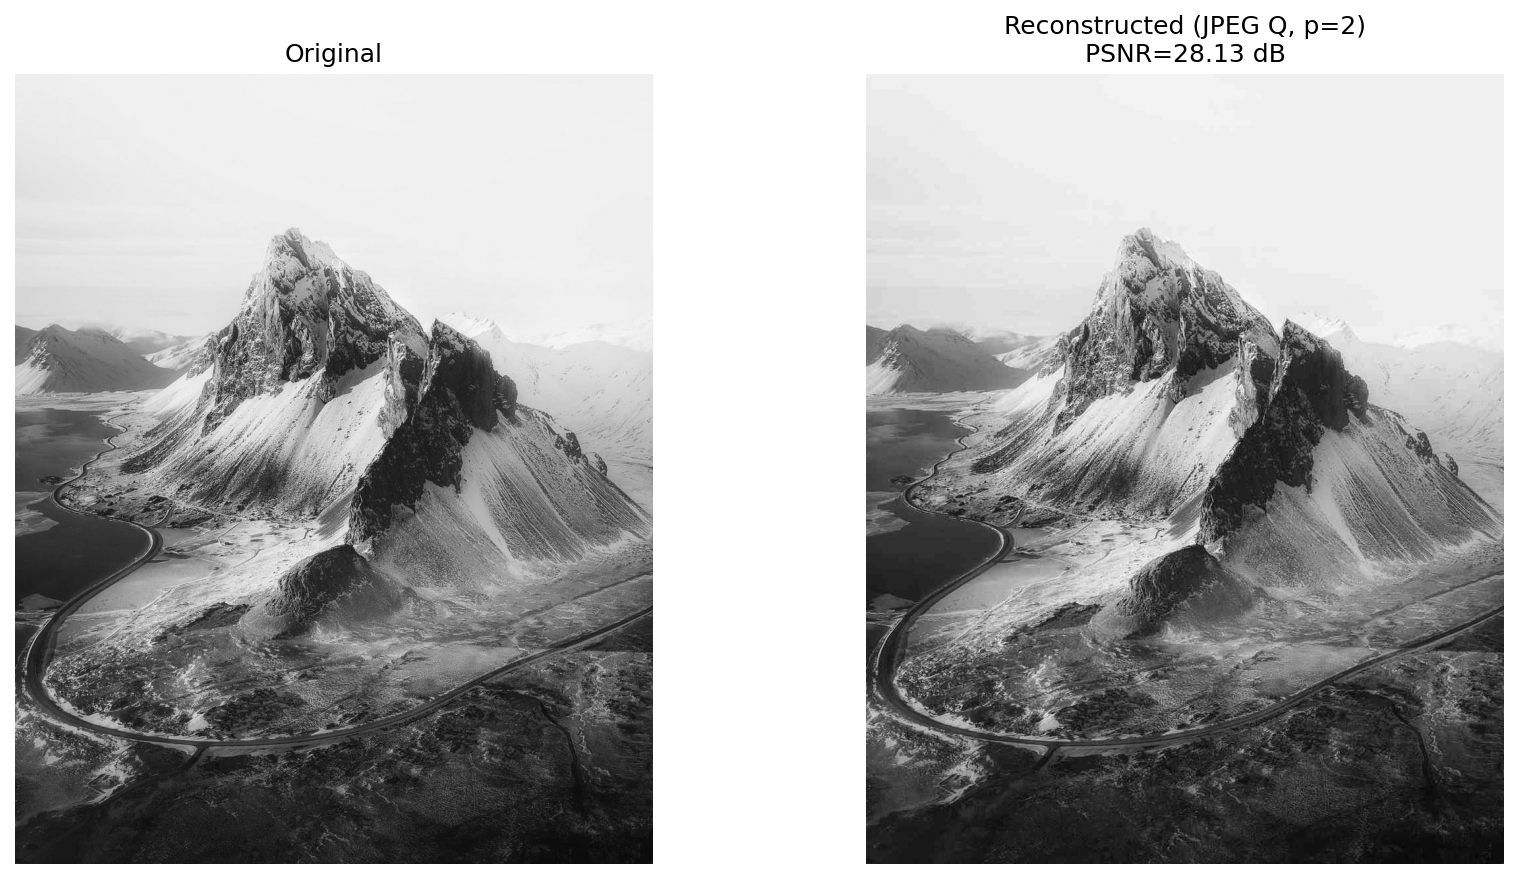
\includegraphics[width=0.48\textwidth]{figures/p3_2_B_p2.png}
  \caption{Reconstruction with JPEG $Q_Y$, $p=2$.}
  \label{fig:b2}
\end{figure}

%--------------------------------------------------
\subsection{Compression Statistics (3.3)}

Tables~\ref{tab:p31} and \ref{tab:p32} summarize the compression statistics for both images under all quantization settings.

\begin{table}[H]
\centering
\caption{Compression statistics for \texttt{p3\_1.png}.}
\label{tab:p31}
\begin{tabular}{lcccccc}
\toprule
Setting & Overall Zero & Low-Freq Zero & High-Freq Zero & PSNR (dB) & RLE Length \\
\midrule
Simple $p=4$    & 0.9547 & 0.8143 & 0.9806 & 46.71 & 173\,534 \\
Simple $p=8$    & 0.9601 & 0.8222 & 0.9857 & 41.61 & 156\,919 \\
Simple $p=16$   & 0.9659 & 0.8294 & 0.9912 & 36.30 & 139\,492 \\
\midrule
JPEG $p=0.5$    & 0.9525 & 0.8088 & 0.9792 & 48.07 & 180\,552 \\
JPEG $p=1$      & 0.9573 & 0.8149 & 0.9837 & 42.82 & 165\,618 \\
JPEG $p=2$      & 0.9632 & 0.8228 & 0.9891 & 37.88 & 148\,381 \\
\bottomrule
\end{tabular}
\end{table}

\begin{table}[H]
\centering
\caption{Compression statistics for \texttt{p3\_2.png}.}
\label{tab:p32}
\begin{tabular}{lcccccc}
\toprule
Setting & Overall Zero & Low-Freq Zero & High-Freq Zero & PSNR (dB) & RLE Length \\
\midrule
Simple $p=4$    & 0.7924 & 0.4536 & 0.8551 & 33.25 & 307\,218 \\
Simple $p=8$    & 0.8804 & 0.5636 & 0.9391 & 29.41 & 189\,540 \\
Simple $p=16$   & 0.9375 & 0.6871 & 0.9839 & 26.63 & 107\,311 \\
\midrule
JPEG $p=0.5$    & 0.7500 & 0.3681 & 0.8207 & 33.98 & 353\,523 \\
JPEG $p=1$      & 0.8315 & 0.4545 & 0.9014 & 30.55 & 248\,287 \\
JPEG $p=2$      & 0.8944 & 0.5649 & 0.9554 & 28.13 & 165\,700 \\
\bottomrule
\end{tabular}
\end{table}

%--------------------------------------------------
\subsection{Zigzag Scan and Run-Length Encoding (3.4)}

The zigzag scan reorders each quantized $8\times 8$ block from low frequency to high frequency.  Since high-frequency coefficients are predominantly zero after quantization, the zigzag ordering clusters zeros together at the end of the sequence, making run-length encoding (RLE) highly effective.

The ``RLE Length'' column in Tables~\ref{tab:p31} and \ref{tab:p32} gives the total number of (value, run-length) pairs across all blocks.

\textbf{Trend:}  Higher zero ratio directly leads to shorter RLE encoded sequences.  As the quantization becomes more aggressive (larger $p$), more coefficients are quantized to zero, producing longer runs of consecutive zeros after zigzag reordering.  Each long run of zeros collapses to a single (0, count) pair in RLE, substantially reducing the encoded length.

%--------------------------------------------------
\subsection{Analysis (3.5)}

\textbf{1. Effect of increasing quantization scale.}
\begin{itemize}[nosep]
  \item \textbf{Visual quality} degrades: blocking artifacts become visible, fine details are lost.
  \item \textbf{Zero ratio} increases: more coefficients are rounded to zero.
  \item \textbf{PSNR} decreases: larger quantization error leads to lower signal-to-noise ratio.
  \item \textbf{Encoded length} (RLE) decreases: more zeros mean longer zero-runs and fewer RLE symbols.
\end{itemize}
This is the fundamental \emph{rate--distortion tradeoff}: higher compression comes at the cost of lower quality.

\medskip
\textbf{2. Simple matrix vs.\ JPEG luminance matrix.}

At comparable zero ratios, the JPEG luminance matrix generally achieves \emph{higher PSNR} than the simple hand-crafted matrix.  For example, on \texttt{p3\_2.png}, JPEG $p=1$ gives zero ratio 0.83 / PSNR 30.55\,dB, while Simple $p=4$ gives zero ratio 0.79 / PSNR 33.25\,dB.  However, comparing at similar aggressiveness levels, the JPEG matrix is better tuned to human perception: it quantizes perceptually unimportant high-frequency coefficients more aggressively while preserving important low-frequency detail, leading to better subjective quality at a given bit rate.  Overall, the JPEG matrix is the superior strategy, as it was carefully designed based on psychovisual experiments.

\medskip
\textbf{3. Does higher zero ratio always imply better perceptual quality?}

No.  A higher zero ratio means more information has been discarded.  While this improves compression, it generally \emph{degrades} perceptual quality.  The relationship depends heavily on \emph{which} coefficients are zeroed.  Zeroing out perceptually unimportant high-frequency coefficients may have minimal visual impact, but if low-frequency or perceptually important mid-frequency coefficients are also zeroed, visible artifacts (blocking, color banding, loss of contrast) appear.  A well-designed quantization matrix can achieve a high zero ratio with acceptable quality by concentrating the zeros in perceptually irrelevant positions.

\medskip
\textbf{4. Which image is easier to compress?}

\texttt{p3\_1.png} is significantly easier to compress.  It is a stylized map graphic with large flat regions, limited color variation, and relatively few edges.  This means most $8\times 8$ blocks have very little high-frequency energy, and the DCT coefficients are concentrated in the DC/low-frequency positions.  Even mild quantization produces a very high zero ratio ($>95\%$) with excellent PSNR ($>40$\,dB).

\texttt{p3\_2.png} is a natural photograph of a mountain with rich texture, continuous tonal gradations, and many fine details (snow, rock, road).  The DCT coefficients spread more broadly across frequencies, making it harder to quantize aggressively without significant quality loss.  At the same quantization settings, \texttt{p3\_2.png} always has lower zero ratio, lower PSNR, and longer RLE sequences than \texttt{p3\_1.png}.

\end{document}
